\documentclass{iopart}
% Uncomment next line if AMS fonts required
\usepackage{iopams}
\usepackage{color}
%Ben inserted the following 7 lines, so graphics would work
%\ifx\pdfoutput\undefined %\usepackage[dvips]{graphicx} %\else
%\usepackage[pdftex]{graphicx} %\pdfcompresslevel=9 %\fi
\usepackage{epstopdf}
\usepackage{latexsym}
\usepackage{amsfonts}
\usepackage{graphicx}
%\usepackage{subfig}
\usepackage{url}
\def\sqr#1#2{$\vcenter{\hrule height.#2pt
\hbox{\vrule width.#2pt height#1pt \kern#1pt \vrule width.#2pt} \hrule
height.#2pt}$}
\def\qed{\sqr53}
\def\mk{\mathcal{K}}
\def\ml{\mathcal{L}}
\def\p{\prime}
\newtheorem{lemma}{Lemma}
\newtheorem{theorem}{Theorem}
\newtheorem{definition}{Definition}
\newtheorem{corollary}{Corollary}
\newcommand{\proof}{\medskip\noindent{\rm\bf Proof. \ }}
\newcommand{\remark}{\bigskip\noindent{\rm\bf Remark.}}

\begin{document}

\title[Estimating the topological complexity of open chains]{Estimating the topological complexity of open chains}

\author{M. Pouokam J. Arsuaga$^\ast$\footnote[1]{To whom correspondence should be addressed
(jarsuaga@ucdavis.edu)}}
\address{$^\ast$Department of Mathematics \& \\
Department of Molecular and Cellular Biology\\
University of California at Davis\\
Davis, CA 95616}

\begin{abstract}
Estimating the topological complexity of closed chains is a well defined problem and can be addressed using several topological invariant including the linking number or standard polynomial invariants. Genomes however are composed of chromosomes that are linear rather than circular. How to measure the entanglement of open chains remains open. Here we propose to estimate the topological entanglement between two open chains using closure methods, as those proposed for measuring the entanglement of proteins. We find that this random closure approach performs better than the linking number for open chains. 
I am testing Git here
this is a mess ...


\end{abstract}

%Uncomment for PACS numbers title message

\ams{57M25 and 92B99.}

% Uncomment for Submitted to journal title message %\submitto{\JPA}

% Comment out if separate title page not required %\maketitle

\section{Introduction}
\begin{figure}[!htb]
\begin{center}
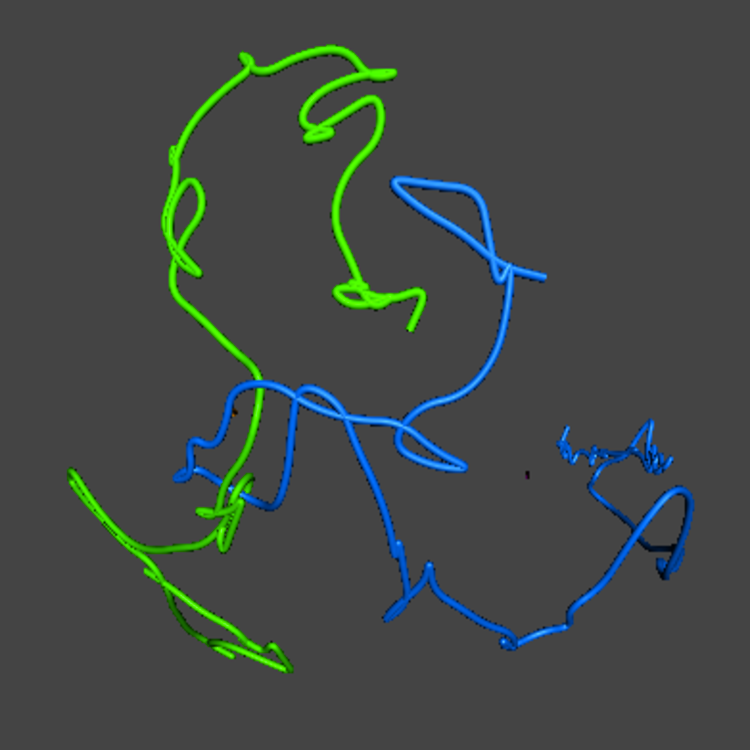
\includegraphics[angle=270,scale=0.23]{Panel7chromo1315}
\includegraphics[angle=270,scale=0.23]{Panel8chrom1315}
\end{center}
\caption{Example of the relative position of two chromosomes.
\label{2Chroms}}
\end{figure}

\section{Methods}

\subsection{Quantification of the entanglement complexity between open chains}
To determine the topological complexity of two open chains $C_1$ and $C_2$ we generated an ensemble of closed circular molecules by using the radial closure method  \cite{Millet2013} (see \ref{examples_closure}) as follows: (1) The centers of masses of each $C_i,i=1,2$, $m_i, i=1,2$, were computed together with the distance between them. (2) Next, for each of the molecules we calculated the smallest radius of the sphere, centered at $m_i$ that contain each of the chains  $R_i,i=1,2$ and a sphere of radius $R+r$ was defined. (3) A set of random points were taken on the surface of the sphere $\{P_i^j\}$ for $i=1,2$ and $j=1,...n$. (3) For each of the chains $C_1$ and $C_2$ an ensemble of circular molecules associated to each of the $C_i$ was defined by connecting the ends of each molecule $C_i$ to each of the points $P_i^j$. (4) The entanglement of the pair of chains $C_i,i=1,2$ was then defined by the linking probability of all the elements of their associated ensembles. IN the calculations presented here the linking number between any two pairs of circular trajectories was  calculated using the gaussian integral form \cite{KL2000}. Results of the linking frequencies were compiled on a lower diagonal triangular matrix. 

%Given the table of pairwise entanglement complexity we tested for statistical significant differences between reconstructions using the Kolmogorov-Smirnov test  on the vectorized form of the matrix $f_{ij}$ \cite{Cornforth2004,Leh,kirk}. The obtained p-values were corrected using FDR \cite{FDR} since a total of  $\choose{12}{2}$ = 66 tests were performed. 

\begin{figure}[!htb]
\begin{center}
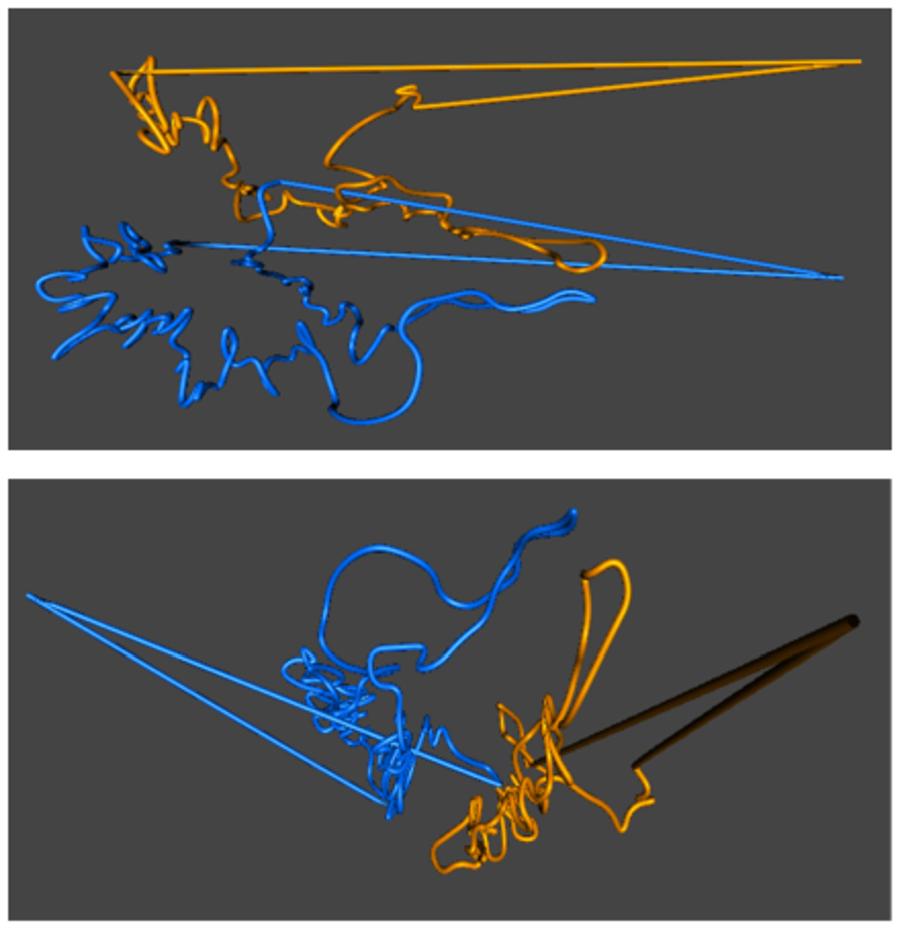
\includegraphics[angle=270,scale=0.35]{Chromo_4-15}
\end{center}
\caption{Random closure of a random walk.
\label{RandomClosure}}
\end{figure}


\medskip


\medskip

\medskip
\section{Numerical results}

\subsection{Dependence of results on the radius of the sphere containing the circularization point} 
Given two open chains we first computed how the results changed when we changed the value of the radius of the sphere containing the set of random points. 

\begin{figure}[!htb]
\begin{center}
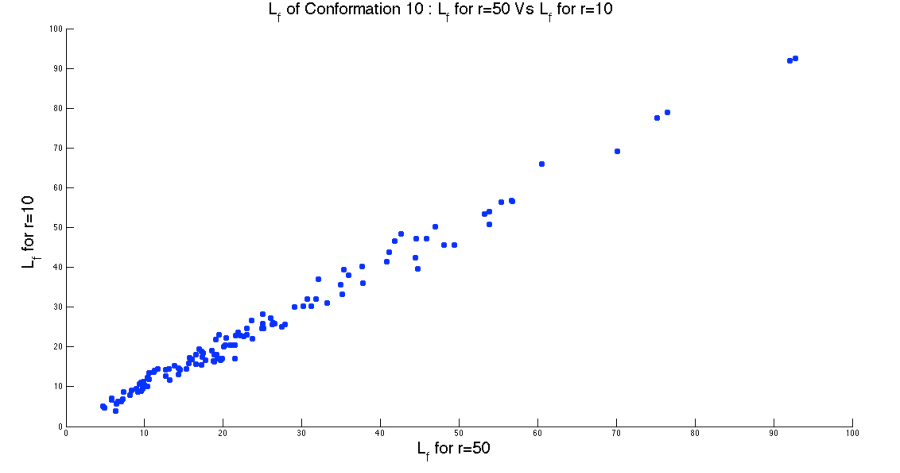
\includegraphics[width=1\textwidth]{L_f-Conf10}
\end{center}
\caption{Results are robust for various radii $r$. the graph shows a high correlation between the linking probability of the pairwise chromosomes in reconstruction 10 for   two different values of $r$, $r=50$ on the x-axis and $r=10$ on the y-axis. the correlation value is $ 0.9941$ \label{fig:L_f-Conf10}}
\end{figure}

To estimate the proportion of closures that gives a specific linking frequency, we investigated the variation of linking frequency versus the number of points sampling. The obvious question one may ask is : how may points are necessary to give an accurate estimate? To address this question we computed the linking frequency of chromosomes 4 and chromosomes 15 from conformation 10.  For comparison, the generated datasets of 10,000, 20,000, 30,000, 40,000, 50,0000 points give linking frequency of 23.06 $\%$, 22.7 $\%$, 22.92$\%$, 22.79$\%$, and 23.07$\%$.  Moreover, using 1,000  closure points in 10 different independent runs we obtained the following linking frequencies 22.10 $\%$, 23.8 $\%$, 22.10 $\%$, 23.1 $\%$, 24.3 $\%$, 22.6 $\%$, 24.0 $\%$, 22.5 $\%$, 22.2 $\%$, 24.9 $\%$ for an average of 23.16 $\%$, which is $ \sim 23.06$ the value obtained  using 10,000 sampling points at once.  Although there is some expected difference between the results (as there would be between random estimates), the data demonstrate the stability of our method. 
Table ~\ref{table:Panel1}  shows the linking frequencies for reconstruction 1 (the other tables can be found in Appendix II). 





\subsection{measure how the values depend with the length}
\subsection{measure how the values depend on distance between the center of masses}
\subsection{ test removing edges from closed molecules}
\subsection{Comparison  with linking number of open curves}
Give example where we detect and the traditional does not. 



%\begin{figure}[!htb]
%\begin{center}
%\includegraphics[angle=270,scale=0.35]{Fig3}
%\end{center}
%\caption{Here goes fig. 3
%\label{Fig3}}
%\end{figure}

%\begin{figure}[!htb]
%\begin{center}
%\includegraphics[angle=270,scale=0.23]{Fig4_1}
%\includegraphics[angle=270,scale=0.23]{Fig4_2}
%\end{center}
%\caption{Here goes to Fig . 4\label{Fig4}}
%\end{figure}


\medskip
\section{Applications}
Yeast again

\medskip
1. Compare different tables not included in the first paper (open linking number) 

\medskip
2. Bonferrroni
\begin{table}[h]
 \caption{p-values for the 12 reconstructions for measures $\phi_D$, $\phi_W$  (upper triangle) and  adjusted p-values of the KS test   (lower triangle). The p-values were adjusted using Bonferroni correction for multiple testing for the 12 reconstructions .}
ÊÊÊÊ\begin{tabular}{l|llllllllllll}
ÊÊÊÊÊÊÊÊ & 1ÊÊÊÊ & 2ÊÊÊÊÊÊÊ & 3ÊÊÊÊ & 4ÊÊÊÊ & 5ÊÊÊÊ & 6ÊÊÊÊ & 7ÊÊÊ & 8ÊÊÊ & 9ÊÊÊ & 10ÊÊ & 11ÊÊ & 12ÊÊ \\ \hline
ÊÊÊÊÊÊÊÊ1Ê & -ÊÊÊÊ &     1.00 & 1.00Ê & 1.00Ê & 1.00Ê & 1.00Ê &  0.00 &  0.00 & 1.00 & 1.00 & 1.00 & 1.00 \\ 
ÊÊÊÊÊÊÊÊ2Ê & 1.00Ê & -ÊÊÊÊÊÊÊ & 1.00Ê & 1.00Ê & 1.00Ê & 1.00Ê &  0.00 &  0.00 & 1.00 & 1.00 & 1.00 & 1.00 \\ 
ÊÊÊÊÊÊÊÊ3Ê & 1.00Ê & 1.00ÊÊÊÊ & -ÊÊÊÊ & 1.00Ê & 1.00Ê & 1.00Ê &  0.00 &  0.04 & 1.00 & 1.00 & 1.00 & 1.00 \\ 
ÊÊÊÊÊÊÊÊ4Ê & 1.00Ê & 1.00ÊÊÊÊ & 1.00Ê & -ÊÊÊÊ & 1.00Ê & 1.00Ê &  0.00 &  0.00 & 1.00 & 1.00 & 1.00 & 1.00 \\ 
ÊÊÊÊÊÊÊÊ5Ê & 1.00Ê & 1.00ÊÊÊÊ & 1.00Ê & 1.00Ê & -ÊÊÊÊ & 1.00Ê &  0.00 &  0.00 & 1.00 & 1.00 & 1.00 & 1.00 \\ 
ÊÊÊÊÊÊÊÊ6Ê & 1.00Ê & 1.00ÊÊÊÊ & 1.00Ê & 1.00Ê & 1.00Ê & -ÊÊÊÊ &  0.00 &  0.00 & 1.00 & 1.00 & 1.00 & 1.00 \\ 
ÊÊÊÊÊÊÊÊ7Ê & 0.066 & 0.462ÊÊÊ & 0.33Ê & 0.132 & 0.462 & 0.594 & -ÊÊÊ & 0.95 & 0.78 &  0.01 &  0.00 &  0.00 \\ 
ÊÊÊÊÊÊÊÊ8Ê & 0.00Ê &  0.00ÊÊÊÊ &  0.00Ê &  0.00Ê & 0.462 & 0.396 & 1.00 & -ÊÊÊ &  0.00 &  0.00 &  0.00 &  0.00 \\ 
ÊÊÊÊÊÊÊÊ9Ê & 0.264 & 0.924ÊÊÊ & 1.00Ê & 1.00Ê &  0.00Ê & 0.066 &  0.00 &  0.00 & -ÊÊÊ & 1.00 & 1.00 & 1.00 \\ 
ÊÊÊÊÊÊÊÊ10 &  0.00Ê &  0.00ÊÊÊÊ &  0.00Ê &  0.00Ê &  0.00Ê &  0.00Ê &  0.00 &  0.00 & 1.00 & -ÊÊÊ & 1.00 & 1.00 \\ 
ÊÊÊÊÊÊÊÊ11 & 0.066 & 1.00ÊÊÊÊ &  0.00Ê &  0.00Ê & 1.00Ê & 1.00Ê & 1.00 & 1.00 &  0.00 &  0.00 & -ÊÊÊ & 1.00 \\ 
ÊÊÊÊÊÊÊÊ12 & 0.924 & 1.00ÊÊÊÊ & 0.924 & 0.594 & 1.00Ê & 1.00Ê & 1.00 & 1.00 &  0.00 &  0.00 & 1.00 & -ÊÊÊ \\
ÊÊÊÊÊÊÊÊ
ÊÊÊÊ\end{tabular}

\label{table:Bonferroni-Correction}
\end{table}

\medskip
3. T

\medskip



\end{document}
